\section{The Ceiling in Each Model, the Matched SAE Comparison and Sparsity at Matched Budgets}\label{app:z}
This section uses the states, dictionaries, centering and bootstrap of Appendix~\ref{app:ci}.
\subsection{Identification and survival in all models}\label{app:z3}
\texttt{exp\_z3\_ceiling} repeats the GPT-2 analysis of Table~\ref{app:survbins} and Table~\ref{app:auc} for the eight models on both corpora: each token's three dominant MLP writes (98,304 cases per model and corpus), their survival $s=(\mathbf{x}\cdot\mathbf{d})/c$ in the observed state, and whether OMP at $k=64$ places the write's atom in the support. Two further quantities decompose the misses. A miss is \emph{erased} if $s<0.25$, \emph{weakened} if $0.25\le s<0.75$, a \emph{twin} miss if the write is intact but an atom within $|\cos|\ge0.95$ of its atom sits in the support instead, and \emph{intact, unselected} otherwise. The GPT-2 row reproduces Table~\ref{app:survbins} exactly.
\begin{table}[H]\centering\scriptsize
\caption{Identification of the three dominant writes on WikiText-2 against their survival. Intact means $s\ge0.75$, erased $s<0.25$. Brackets are 95\% bootstrap intervals over sequences.}\label{app:z3-surv-wikitext}
\begin{adjustbox}{max width=\linewidth}
\begin{tabular}{lrrrrrrrr}\toprule
Model & gated & identified, all cases & share intact & identified, intact & share erased & identified, erased & AUC survival & AUC prominence \\ \midrule
GPT-2 small & no & 0.491 [0.484, 0.497] & 0.834 & 0.584 [0.577, 0.590] & 0.128 & 0.008 [0.007, 0.009] & 0.73 & 0.80 \\
SmolLM2-135M & yes & 0.494 [0.490, 0.497] & 0.761 & 0.614 [0.610, 0.618] & 0.089 & 0.015 [0.013, 0.018] & 0.81 & 0.86 \\
Qwen2.5-0.5B & yes & 0.349 [0.345, 0.353] & 0.527 & 0.550 [0.545, 0.556] & 0.104 & 0.004 [0.003, 0.006] & 0.83 & 0.92 \\
Pythia-410m & no & 0.365 [0.358, 0.371] & 0.762 & 0.465 [0.457, 0.471] & 0.080 & 0.003 [0.002, 0.004] & 0.84 & 0.91 \\
OLMo-1B & yes & 0.606 [0.602, 0.611] & 0.637 & 0.788 [0.782, 0.793] & 0.063 & 0.036 [0.030, 0.041] & 0.82 & 0.89 \\
Qwen2.5-7B & yes & 0.556 [0.547, 0.565] & 0.363 & 0.778 [0.770, 0.787] & 0.094 & 0.076 [0.067, 0.085] & 0.76 & 0.88 \\
Llama-7B & yes & 0.946 [0.944, 0.949] & 0.976 & 0.962 [0.960, 0.963] & 0.009 & 0.150 [0.122, 0.178] & 0.76 & 0.85 \\
Pythia-6.9B & no & 0.687 [0.680, 0.694] & 0.922 & 0.744 [0.737, 0.750] & 0.062 & 0.007 [0.005, 0.009] & 0.82 & 0.86 \\
\bottomrule\end{tabular}\end{adjustbox}
\end{table}
\begin{table}[H]\centering\scriptsize
\caption{Where the misses come from on WikiText-2: the share of missed dominant writes in each class (the four shares sum to one).}\label{app:z3-miss-wikitext}
\begin{adjustbox}{max width=\linewidth}
\begin{tabular}{lrrrrrr}\toprule
Model & miss rate & erased & weakened & twin in support & intact, unselected & cases with a twin in the support \\ \midrule
GPT-2 small & 0.509 & 0.25 [0.24, 0.26] & 0.07 [0.07, 0.07] & 0.00 [0.00, 0.00] & 0.68 [0.67, 0.69] & 0.2\% \\
SmolLM2-135M & 0.506 & 0.17 [0.17, 0.18] & 0.25 [0.24, 0.25] & 0.00 [0.00, 0.00] & 0.58 [0.57, 0.59] & 0.4\% \\
Qwen2.5-0.5B & 0.651 & 0.16 [0.15, 0.16] & 0.48 [0.47, 0.48] & 0.00 [0.00, 0.00] & 0.36 [0.35, 0.37] & 0.1\% \\
Pythia-410m & 0.635 & 0.13 [0.12, 0.13] & 0.23 [0.23, 0.24] & 0.01 [0.01, 0.01] & 0.64 [0.63, 0.64] & 0.3\% \\
OLMo-1B & 0.394 & 0.15 [0.15, 0.16] & 0.50 [0.49, 0.51] & 0.00 [0.00, 0.00] & 0.34 [0.33, 0.35] & 0.1\% \\
Qwen2.5-7B & 0.444 & 0.20 [0.19, 0.20] & 0.62 [0.61, 0.63] & 0.00 [0.00, 0.00] & 0.18 [0.17, 0.19] & 0.2\% \\
Llama-7B & 0.054 & 0.14 [0.12, 0.15] & 0.17 [0.16, 0.18] & 0.01 [0.01, 0.01] & 0.69 [0.67, 0.70] & 0.4\% \\
Pythia-6.9B & 0.313 & 0.20 [0.19, 0.21] & 0.05 [0.05, 0.05] & 0.00 [0.00, 0.00] & 0.75 [0.74, 0.76] & 0.0\% \\
\bottomrule\end{tabular}\end{adjustbox}
\end{table}
\begin{table}[H]\centering\scriptsize
\caption{OMP identification rate by survival bin on WikiText-2 (the six bins of Figure~\ref{fig:fvu}).}\label{app:z3-bins-wikitext}
\begin{adjustbox}{max width=\linewidth}
\begin{tabular}{lrrrrrr}\toprule
Model & $s<0$ & $[0,0.25)$ & $[0.25,0.5)$ & $[0.5,0.75)$ & $[0.75,1.25)$ & $s\ge1.25$ \\ \midrule
GPT-2 small & 0.01 & 0.01 & 0.04 & 0.11 & 0.36 & 0.62 \\
SmolLM2-135M & 0.01 & 0.04 & 0.08 & 0.22 & 0.38 & 0.71 \\
Qwen2.5-0.5B & 0.00 & 0.01 & 0.10 & 0.20 & 0.36 & 0.73 \\
Pythia-410m & 0.00 & 0.00 & 0.02 & 0.09 & 0.22 & 0.62 \\
OLMo-1B & 0.06 & 0.02 & 0.15 & 0.45 & 0.72 & 0.88 \\
Qwen2.5-7B & 0.03 & 0.08 & 0.38 & 0.60 & 0.75 & 0.85 \\
Llama-7B & 0.15 & 0.15 & 0.26 & 0.51 & 0.84 & 0.97 \\
Pythia-6.9B & 0.01 & 0.01 & 0.02 & 0.03 & 0.10 & 0.77 \\
\bottomrule\end{tabular}\end{adjustbox}
\end{table}
\begin{figure}[H]\centering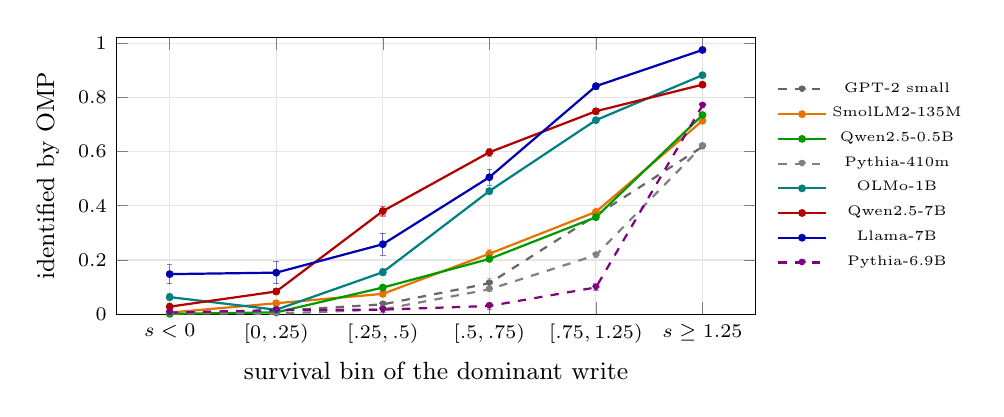
\begin{tikzpicture}\begin{axis}[width=0.8\linewidth, height=0.42\linewidth, xlabel={survival bin of the dominant write}, ylabel={identified by OMP}, xmin=0.5, xmax=6.5, ymin=0, ymax=1.02, xtick={1,...,6}, xticklabels={{$s<0$},{$[0,.25)$},{$[.25,.5)$},{$[.5,.75)$},{$[.75,1.25)$},{$s\ge1.25$}}, grid=major, grid style={black!10}, legend style={font=\tiny, at={(1.02,0.5)}, anchor=west, draw=none}, tick label style={font=\scriptsize}, label style={font=\small}, error bars/y dir=both, error bars/y explicit]
\addplot[thick, dashed, color=black!60, mark=*, mark size=1pt, error bars/error bar style={opacity=0.5}] coordinates {(1,0.0074) +- (0,0.0013) (2,0.0122) +- (0,0.0058) (3,0.0362) +- (0,0.0101) (4,0.1141) +- (0,0.0166) (5,0.3644) +- (0,0.0106) (6,0.6178) +- (0,0.0066)};\addlegendentry{GPT-2 small}
\addplot[thick, color=orange!90!black, mark=*, mark size=1pt, error bars/error bar style={opacity=0.5}] coordinates {(1,0.0058) +- (0,0.0018) (2,0.0404) +- (0,0.0087) (3,0.0750) +- (0,0.0083) (4,0.2229) +- (0,0.0152) (5,0.3774) +- (0,0.0100) (6,0.7137) +- (0,0.0057)};\addlegendentry{SmolLM2-135M}
\addplot[thick, color=green!60!black, mark=*, mark size=1pt, error bars/error bar style={opacity=0.5}] coordinates {(1,0.0012) +- (0,0.0012) (2,0.0067) +- (0,0.0025) (3,0.0982) +- (0,0.0088) (4,0.2038) +- (0,0.0088) (5,0.3578) +- (0,0.0066) (6,0.7346) +- (0,0.0074)};\addlegendentry{Qwen2.5-0.5B}
\addplot[thick, dashed, color=gray, mark=*, mark size=1pt, error bars/error bar style={opacity=0.5}] coordinates {(1,0.0039) +- (0,0.0018) (2,0.0015) +- (0,0.0015) (3,0.0179) +- (0,0.0031) (4,0.0917) +- (0,0.0062) (5,0.2178) +- (0,0.0081) (6,0.6207) +- (0,0.0097)};\addlegendentry{Pythia-410m}
\addplot[thick, color=teal, mark=*, mark size=1pt, error bars/error bar style={opacity=0.5}] coordinates {(1,0.0630) +- (0,0.0116) (2,0.0164) +- (0,0.0052) (3,0.1548) +- (0,0.0121) (4,0.4543) +- (0,0.0110) (5,0.7158) +- (0,0.0074) (6,0.8817) +- (0,0.0051)};\addlegendentry{OLMo-1B}
\addplot[thick, color=red!70!black, mark=*, mark size=1pt, error bars/error bar style={opacity=0.5}] coordinates {(1,0.0277) +- (0,0.0110) (2,0.0837) +- (0,0.0097) (3,0.3803) +- (0,0.0182) (4,0.5972) +- (0,0.0142) (5,0.7487) +- (0,0.0105) (6,0.8468) +- (0,0.0073)};\addlegendentry{Qwen2.5-7B}
\addplot[thick, color=blue!70!black, mark=*, mark size=1pt, error bars/error bar style={opacity=0.5}] coordinates {(1,0.1478) +- (0,0.0349) (2,0.1532) +- (0,0.0413) (3,0.2581) +- (0,0.0411) (4,0.5052) +- (0,0.0290) (5,0.8413) +- (0,0.0108) (6,0.9748) +- (0,0.0014)};\addlegendentry{Llama-7B}
\addplot[thick, dashed, color=violet, mark=*, mark size=1pt, error bars/error bar style={opacity=0.5}] coordinates {(1,0.0060) +- (0,0.0021) (2,0.0149) +- (0,0.0090) (3,0.0168) +- (0,0.0099) (4,0.0303) +- (0,0.0131) (5,0.0987) +- (0,0.0125) (6,0.7697) +- (0,0.0057)};\addlegendentry{Pythia-6.9B}
\end{axis}\end{tikzpicture}\caption{Identification against survival for all eight models on WikiText-2. Solid lines are gated-MLP models, dashed non-gated.}\label{app:z3-fig-wikitext}\end{figure}
\begin{table}[H]\centering\scriptsize
\caption{Identification of the three dominant writes on the Pile sample against their survival. Intact means $s\ge0.75$, erased $s<0.25$. Brackets are 95\% bootstrap intervals over sequences.}\label{app:z3-surv-pile}
\begin{adjustbox}{max width=\linewidth}
\begin{tabular}{lrrrrrrrr}\toprule
Model & gated & identified, all cases & share intact & identified, intact & share erased & identified, erased & AUC survival & AUC prominence \\ \midrule
GPT-2 small & no & 0.439 [0.423, 0.454] & 0.765 & 0.571 [0.560, 0.581] & 0.187 & 0.007 [0.005, 0.009] & 0.80 & 0.83 \\
SmolLM2-135M & yes & 0.489 [0.479, 0.497] & 0.794 & 0.594 [0.587, 0.601] & 0.082 & 0.010 [0.008, 0.012] & 0.81 & 0.88 \\
Qwen2.5-0.5B & yes & 0.365 [0.355, 0.375] & 0.573 & 0.551 [0.544, 0.559] & 0.093 & 0.002 [0.001, 0.003] & 0.84 & 0.92 \\
Pythia-410m & no & 0.346 [0.337, 0.353] & 0.735 & 0.454 [0.446, 0.461] & 0.084 & 0.004 [0.002, 0.008] & 0.83 & 0.91 \\
OLMo-1B & yes & 0.639 [0.632, 0.647] & 0.704 & 0.778 [0.771, 0.786] & 0.043 & 0.027 [0.021, 0.033] & 0.79 & 0.87 \\
Qwen2.5-7B & yes & 0.578 [0.567, 0.588] & 0.475 & 0.761 [0.750, 0.772] & 0.069 & 0.068 [0.060, 0.077] & 0.75 & 0.87 \\
Llama-7B & yes & 0.948 [0.944, 0.951] & 0.977 & 0.962 [0.960, 0.964] & 0.008 & 0.112 [0.093, 0.134] & 0.75 & 0.84 \\
Pythia-6.9B & no & 0.669 [0.656, 0.681] & 0.915 & 0.730 [0.718, 0.741] & 0.072 & 0.010 [0.007, 0.013] & 0.80 & 0.80 \\
\bottomrule\end{tabular}\end{adjustbox}
\end{table}
\begin{table}[H]\centering\scriptsize
\caption{Where the misses come from on the Pile sample: the share of missed dominant writes in each class (the four shares sum to one).}\label{app:z3-miss-pile}
\begin{adjustbox}{max width=\linewidth}
\begin{tabular}{lrrrrrr}\toprule
Model & miss rate & erased & weakened & twin in support & intact, unselected & cases with a twin in the support \\ \midrule
GPT-2 small & 0.561 & 0.33 [0.30, 0.37] & 0.08 [0.08, 0.09] & 0.00 [0.00, 0.00] & 0.58 [0.55, 0.61] & 0.3\% \\
SmolLM2-135M & 0.511 & 0.16 [0.15, 0.17] & 0.21 [0.20, 0.22] & 0.00 [0.00, 0.00] & 0.63 [0.62, 0.64] & 0.3\% \\
Qwen2.5-0.5B & 0.635 & 0.15 [0.14, 0.15] & 0.45 [0.43, 0.46] & 0.00 [0.00, 0.00] & 0.40 [0.39, 0.42] & 0.1\% \\
Pythia-410m & 0.654 & 0.13 [0.12, 0.14] & 0.26 [0.25, 0.27] & 0.01 [0.00, 0.01] & 0.61 [0.60, 0.62] & 0.3\% \\
OLMo-1B & 0.361 & 0.12 [0.11, 0.12] & 0.45 [0.44, 0.46] & 0.00 [0.00, 0.00] & 0.43 [0.41, 0.44] & 0.1\% \\
Qwen2.5-7B & 0.422 & 0.15 [0.15, 0.16] & 0.58 [0.57, 0.59] & 0.00 [0.00, 0.00] & 0.26 [0.25, 0.28] & 0.2\% \\
Llama-7B & 0.052 & 0.14 [0.13, 0.16] & 0.15 [0.14, 0.17] & 0.01 [0.01, 0.01] & 0.70 [0.67, 0.72] & 0.4\% \\
Pythia-6.9B & 0.331 & 0.22 [0.20, 0.23] & 0.04 [0.04, 0.04] & 0.00 [0.00, 0.00] & 0.74 [0.73, 0.76] & 0.1\% \\
\bottomrule\end{tabular}\end{adjustbox}
\end{table}
\begin{table}[H]\centering\scriptsize
\caption{OMP identification rate by survival bin on the Pile sample (the six bins of Figure~\ref{fig:fvu}).}\label{app:z3-bins-pile}
\begin{adjustbox}{max width=\linewidth}
\begin{tabular}{lrrrrrr}\toprule
Model & $s<0$ & $[0,0.25)$ & $[0.25,0.5)$ & $[0.5,0.75)$ & $[0.75,1.25)$ & $s\ge1.25$ \\ \midrule
GPT-2 small & 0.01 & 0.00 & 0.01 & 0.05 & 0.24 & 0.62 \\
SmolLM2-135M & 0.00 & 0.02 & 0.08 & 0.16 & 0.33 & 0.70 \\
Qwen2.5-0.5B & 0.00 & 0.00 & 0.08 & 0.20 & 0.36 & 0.74 \\
Pythia-410m & 0.00 & 0.00 & 0.01 & 0.09 & 0.23 & 0.61 \\
OLMo-1B & 0.02 & 0.03 & 0.17 & 0.45 & 0.71 & 0.86 \\
Qwen2.5-7B & 0.06 & 0.07 & 0.35 & 0.55 & 0.72 & 0.83 \\
Llama-7B & 0.08 & 0.17 & 0.37 & 0.51 & 0.81 & 0.97 \\
Pythia-6.9B & 0.01 & 0.01 & 0.03 & 0.05 & 0.11 & 0.75 \\
\bottomrule\end{tabular}\end{adjustbox}
\end{table}
\begin{figure}[H]\centering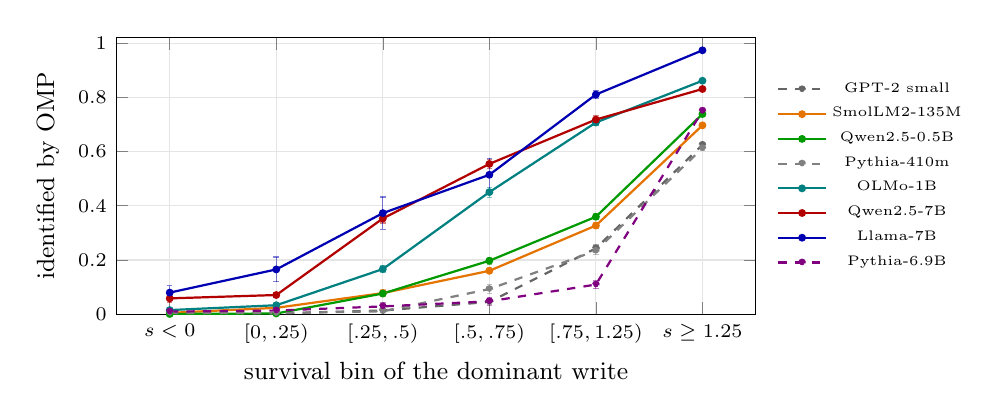
\begin{tikzpicture}\begin{axis}[width=0.8\linewidth, height=0.42\linewidth, xlabel={survival bin of the dominant write}, ylabel={identified by OMP}, xmin=0.5, xmax=6.5, ymin=0, ymax=1.02, xtick={1,...,6}, xticklabels={{$s<0$},{$[0,.25)$},{$[.25,.5)$},{$[.5,.75)$},{$[.75,1.25)$},{$s\ge1.25$}}, grid=major, grid style={black!10}, legend style={font=\tiny, at={(1.02,0.5)}, anchor=west, draw=none}, tick label style={font=\scriptsize}, label style={font=\small}, error bars/y dir=both, error bars/y explicit]
\addplot[thick, dashed, color=black!60, mark=*, mark size=1pt, error bars/error bar style={opacity=0.5}] coordinates {(1,0.0074) +- (0,0.0019) (2,0.0028) +- (0,0.0023) (3,0.0136) +- (0,0.0060) (4,0.0453) +- (0,0.0102) (5,0.2429) +- (0,0.0125) (6,0.6247) +- (0,0.0097)};\addlegendentry{GPT-2 small}
\addplot[thick, color=orange!90!black, mark=*, mark size=1pt, error bars/error bar style={opacity=0.5}] coordinates {(1,0.0048) +- (0,0.0018) (2,0.0234) +- (0,0.0072) (3,0.0778) +- (0,0.0116) (4,0.1600) +- (0,0.0111) (5,0.3270) +- (0,0.0102) (6,0.6967) +- (0,0.0071)};\addlegendentry{SmolLM2-135M}
\addplot[thick, color=green!60!black, mark=*, mark size=1pt, error bars/error bar style={opacity=0.5}] coordinates {(1,0.0008) +- (0,0.0008) (2,0.0025) +- (0,0.0014) (3,0.0762) +- (0,0.0085) (4,0.1971) +- (0,0.0128) (5,0.3594) +- (0,0.0108) (6,0.7383) +- (0,0.0077)};\addlegendentry{Qwen2.5-0.5B}
\addplot[thick, dashed, color=gray, mark=*, mark size=1pt, error bars/error bar style={opacity=0.5}] coordinates {(1,0.0048) +- (0,0.0050) (2,0.0037) +- (0,0.0026) (3,0.0107) +- (0,0.0024) (4,0.0926) +- (0,0.0157) (5,0.2339) +- (0,0.0150) (6,0.6123) +- (0,0.0085)};\addlegendentry{Pythia-410m}
\addplot[thick, color=teal, mark=*, mark size=1pt, error bars/error bar style={opacity=0.5}] coordinates {(1,0.0151) +- (0,0.0081) (2,0.0330) +- (0,0.0074) (3,0.1664) +- (0,0.0120) (4,0.4503) +- (0,0.0183) (5,0.7072) +- (0,0.0107) (6,0.8613) +- (0,0.0070)};\addlegendentry{OLMo-1B}
\addplot[thick, color=red!70!black, mark=*, mark size=1pt, error bars/error bar style={opacity=0.5}] coordinates {(1,0.0583) +- (0,0.0153) (2,0.0707) +- (0,0.0097) (3,0.3530) +- (0,0.0167) (4,0.5544) +- (0,0.0170) (5,0.7180) +- (0,0.0146) (6,0.8308) +- (0,0.0107)};\addlegendentry{Qwen2.5-7B}
\addplot[thick, color=blue!70!black, mark=*, mark size=1pt, error bars/error bar style={opacity=0.5}] coordinates {(1,0.0796) +- (0,0.0247) (2,0.1651) +- (0,0.0458) (3,0.3728) +- (0,0.0596) (4,0.5143) +- (0,0.0604) (5,0.8104) +- (0,0.0148) (6,0.9735) +- (0,0.0014)};\addlegendentry{Llama-7B}
\addplot[thick, dashed, color=violet, mark=*, mark size=1pt, error bars/error bar style={opacity=0.5}] coordinates {(1,0.0096) +- (0,0.0028) (2,0.0133) +- (0,0.0105) (3,0.0287) +- (0,0.0143) (4,0.0475) +- (0,0.0150) (5,0.1093) +- (0,0.0148) (6,0.7500) +- (0,0.0121)};\addlegendentry{Pythia-6.9B}
\end{axis}\end{tikzpicture}\caption{Identification against survival for all eight models on the Pile sample. Solid lines are gated-MLP models, dashed non-gated.}\label{app:z3-fig-pile}\end{figure}
\begin{table}[H]\centering\scriptsize
\caption{Composition of the $k=64$ support by atom type on WikiText-2.}\label{app:z3-support}
\begin{adjustbox}{max width=\linewidth}
\begin{tabular}{lrrrr}\toprule
Model & embedding & MLP & attention & bias \\ \midrule
GPT-2 small & 17.1\% & 62.1\% & 20.7\% & 0.1\% \\
SmolLM2-135M & 8.5\% & 71.4\% & 20.1\% & 0.0\% \\
Qwen2.5-0.5B & 36.4\% & 54.5\% & 9.1\% & 0.0\% \\
Pythia-410m & 32.8\% & 53.4\% & 13.8\% & 0.0\% \\
OLMo-1B & 16.1\% & 70.4\% & 13.5\% & 0.0\% \\
Qwen2.5-7B & 6.8\% & 80.5\% & 12.7\% & 0.0\% \\
Llama-7B & 2.0\% & 76.9\% & 21.1\% & 0.0\% \\
Pythia-6.9B & 3.9\% & 70.9\% & 25.2\% & 0.0\% \\
\bottomrule\end{tabular}\end{adjustbox}
\end{table}
\subsection{The SAE comparison on identical states}\label{app:z4}
\texttt{exp\_z4\_sae} evaluates the residual-stream SAEs of \citet{bloom2024} from their published weights and the weight dictionary on the same GPT-2 states in four cells: WikiText-2 with 512-token contexts (the paper's states) and OpenWebText with 128-token contexts and a leading beginning-of-text token (the SAEs' training convention), each at the state after block 5 (the input of block 6, where the SAE named \texttt{blocks.6} was trained) and after block 6 (the paper's layer, where \texttt{blocks.7} was trained). The SAEs read the residual stream in the TransformerLens frame, in which each state is centered over the model dimension, and the states are centered the same way before encoding. $L_0$ is the SAE's mean number of active features over the typical states; the weight dictionary is run at $k=32$, $k=64$ and at $k$ equal to that $L_0$. FVU is over the typical states with one denominator per cell for both methods (for GPT-2 the sink states are exactly the first positions), and $\Delta$CE is the change in next-token cross-entropy over all positions when the reconstruction replaces the state in the forward pass. On the 512-token states the SAE fails past position 127, which it never saw in training, so the two 128-token cells are the matched comparison.
\begin{table}[H]\centering\scriptsize
\caption{The trained SAE and the weight dictionary on identical GPT-2 states. Brackets are 95\% bootstrap intervals over sequences (64 WikiText-2 sequences, 256 OpenWebText documents).}\label{app:z4-table}
\begin{adjustbox}{max width=\linewidth}
\begin{tabular}{llrlrrr}\toprule
Corpus, context & state & clean CE & method & $L_0$ or $k$ & FVU, typical states & $\Delta$CE \\ \midrule
WikiText-2, 512 & after block 5 & 3.647 & SAE & 161.6 & 2.878 [2.757, 3.006] & 1.443 [1.390, 1.492] \\
 &  &  & weight dictionary & 32 & 0.325 [0.324, 0.327] & 0.521 [0.495, 0.548] \\
 &  &  & weight dictionary & 64 & 0.174 [0.173, 0.174] & 0.161 [0.150, 0.171] \\
 &  &  & weight dictionary & 162 & 0.023 [0.023, 0.023] & 0.013 [0.011, 0.015] \\
WikiText-2, 512 & after block 6 & 3.647 & SAE & 161.4 & 1.480 [1.422, 1.540] & 1.088 [1.044, 1.131] \\
 &  &  & weight dictionary & 32 & 0.338 [0.337, 0.340] & 0.551 [0.522, 0.581] \\
 &  &  & weight dictionary & 64 & 0.179 [0.179, 0.180] & 0.178 [0.167, 0.189] \\
 &  &  & weight dictionary & 161 & 0.024 [0.024, 0.024] & 0.015 [0.013, 0.017] \\
OpenWebText, 128 & after block 5 & 3.323 & SAE & 51.2 & 0.109 [0.107, 0.111] & 0.144 [0.135, 0.155] \\
 &  &  & weight dictionary & 32 & 0.307 [0.306, 0.308] & 0.428 [0.411, 0.448] \\
 &  &  & weight dictionary & 51 & 0.210 [0.209, 0.211] & 0.188 [0.179, 0.197] \\
 &  &  & weight dictionary & 64 & 0.163 [0.162, 0.164] & 0.125 [0.118, 0.132] \\
OpenWebText, 128 & after block 6 & 3.323 & SAE & 58.8 & 0.121 [0.119, 0.123] & 0.155 [0.145, 0.165] \\
 &  &  & weight dictionary & 32 & 0.320 [0.319, 0.321] & 0.477 [0.460, 0.497] \\
 &  &  & weight dictionary & 59 & 0.187 [0.186, 0.187] & 0.172 [0.165, 0.181] \\
 &  &  & weight dictionary & 64 & 0.169 [0.169, 0.170] & 0.146 [0.138, 0.154] \\
\bottomrule\end{tabular}\end{adjustbox}
\end{table}
\subsection{Sparsity at matched budgets}\label{app:z5}
\texttt{exp\_z5\_kcurve} sweeps $k$ for the weight dictionary and its rotation on 8,192 WikiText-2 states per model (the first 16 evaluation sequences of the sweep), reading the FVU at $k=4$ to $256$ and at the matched budgets $k=d/16$ and $k=d/12$, so that models of different width are compared at the same fraction of their dimension. The table and the figure are over the typical states.
\begin{table}[H]\centering\scriptsize
\caption{FVU of the typical states at a fixed budget of 32 atoms, at budgets matched to the width, and at 256 atoms.}\label{app:z5-table}
\begin{adjustbox}{max width=\linewidth}
\begin{tabular}{lrrrrrrrrrrr}\toprule
Model & $d$ & weight, $k=32$ & rotated, $k=32$ & $k=d/16$ & weight & rotated & $k=d/12$ & weight & rotated & weight, $k=256$ & rotated, $k=256$ \\ \midrule
GPT-2 small & 768 & 0.334 & 0.530 & 48 & 0.243 & 0.391 & 64 & 0.177 & 0.288 & 0.002 & 0.004 \\
SmolLM2-135M & 576 & 0.270 & 0.421 & 36 & 0.242 & 0.379 & 48 & 0.175 & 0.276 & 0.000 & 0.000 \\
Qwen2.5-0.5B & 896 & 0.407 & 0.527 & 56 & 0.255 & 0.330 & 74 & 0.180 & 0.231 & 0.003 & 0.004 \\
Pythia-410m & 1024 & 0.501 & 0.592 & 64 & 0.301 & 0.359 & 85 & 0.216 & 0.257 & 0.010 & 0.013 \\
OLMo-1B & 2048 & 0.564 & 0.773 & 128 & 0.269 & 0.382 & 170 & 0.197 & 0.280 & 0.102 & 0.145 \\
Qwen2.5-7B & 3584 & 0.543 & 0.847 & 224 & 0.210 & 0.351 & 298 & 0.150 & 0.249 & 0.182 & 0.303 \\
Llama-7B & 4096 & 0.621 & 0.872 & 256 & 0.245 & 0.380 & 341 & 0.178 & 0.277 & 0.245 & 0.380 \\
Pythia-6.9B & 4096 & 0.707 & 0.868 & 256 & 0.279 & 0.363 & 341 & 0.199 & 0.260 & 0.279 & 0.363 \\
\bottomrule\end{tabular}\end{adjustbox}
\end{table}
\begin{figure}[H]\centering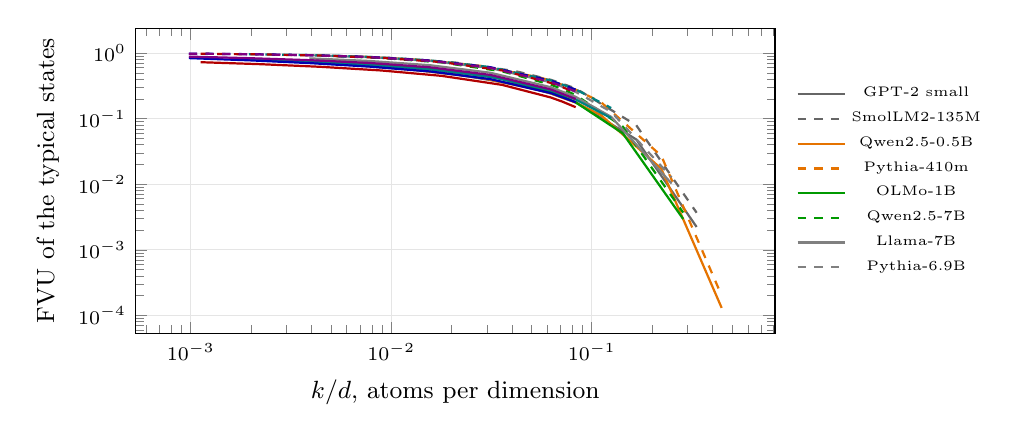
\begin{tikzpicture}\begin{axis}[width=0.8\linewidth, height=0.45\linewidth, xmode=log, ymode=log, xlabel={$k/d$, atoms per dimension}, ylabel={FVU of the typical states}, grid=major, grid style={black!10}, legend style={font=\tiny, at={(1.02,0.5)}, anchor=west, draw=none}, tick label style={font=\scriptsize}, label style={font=\small}]
\addplot[thick, color=black!60, mark=none] coordinates {(0.00521,0.70182) (0.01042,0.59594) (0.02083,0.47543) (0.04167,0.33432) (0.06250,0.24267) (0.08333,0.17722) (0.16667,0.04821) (0.33333,0.00223)};\addlegendentry{GPT-2 small}
\addplot[thick, dashed, color=black!60, mark=none] coordinates {(0.00521,0.91273) (0.01042,0.84044) (0.02083,0.71841) (0.04167,0.52985) (0.06250,0.39147) (0.08333,0.28833) (0.16667,0.07938) (0.33333,0.00368)};
\addplot[thick, color=orange!90!black, mark=none] coordinates {(0.00694,0.64552) (0.01389,0.54337) (0.02778,0.42082) (0.05556,0.26965) (0.06250,0.24208) (0.08333,0.17527) (0.11111,0.11340) (0.22222,0.01721) (0.44444,0.00013)};\addlegendentry{SmolLM2-135M}
\addplot[thick, dashed, color=orange!90!black, mark=none] coordinates {(0.00694,0.88485) (0.01389,0.79223) (0.02778,0.64034) (0.05556,0.42137) (0.06250,0.37931) (0.08333,0.27592) (0.11111,0.17888) (0.22222,0.02713) (0.44444,0.00020)};
\addplot[thick, color=green!60!black, mark=none] coordinates {(0.00446,0.76610) (0.00893,0.67655) (0.01786,0.56148) (0.03571,0.40654) (0.06250,0.25531) (0.07143,0.21853) (0.08259,0.17964) (0.14286,0.05966) (0.28571,0.00295)};\addlegendentry{Qwen2.5-0.5B}
\addplot[thick, dashed, color=green!60!black, mark=none] coordinates {(0.00446,0.91490) (0.00893,0.84295) (0.01786,0.71948) (0.03571,0.52720) (0.06250,0.33011) (0.07143,0.28188) (0.08259,0.23100) (0.14286,0.07562) (0.28571,0.00369)};
\addplot[thick, color=gray, mark=none] coordinates {(0.00391,0.83108) (0.00781,0.75796) (0.01562,0.65336) (0.03125,0.50108) (0.06250,0.30149) (0.08301,0.21573) (0.12500,0.10653) (0.25000,0.01027)};\addlegendentry{Pythia-410m}
\addplot[thick, dashed, color=gray, mark=none] coordinates {(0.00391,0.92772) (0.00781,0.86685) (0.01562,0.76126) (0.03125,0.59174) (0.06250,0.35859) (0.08301,0.25691) (0.12500,0.12712) (0.25000,0.01278)};
\addplot[thick, color=teal, mark=none] coordinates {(0.00195,0.81035) (0.00391,0.73906) (0.00781,0.65963) (0.01562,0.56372) (0.03125,0.43529) (0.06250,0.26923) (0.08301,0.19676) (0.12500,0.10192)};\addlegendentry{OLMo-1B}
\addplot[thick, dashed, color=teal, mark=none] coordinates {(0.00195,0.96293) (0.00391,0.93095) (0.00781,0.87330) (0.01562,0.77300) (0.03125,0.61051) (0.06250,0.38237) (0.08301,0.28012) (0.12500,0.14530)};
\addplot[thick, color=red!70!black, mark=none] coordinates {(0.00112,0.72614) (0.00223,0.67718) (0.00446,0.61711) (0.00893,0.54290) (0.01786,0.44912) (0.03571,0.32752) (0.06250,0.21035) (0.07143,0.18162) (0.08315,0.14961)};\addlegendentry{Qwen2.5-7B}
\addplot[thick, dashed, color=red!70!black, mark=none] coordinates {(0.00112,0.97601) (0.00223,0.95493) (0.00446,0.91628) (0.00893,0.84715) (0.01786,0.72894) (0.03571,0.54395) (0.06250,0.35087) (0.07143,0.30268) (0.08315,0.24890)};
\addplot[thick, color=blue!70!black, mark=none] coordinates {(0.00098,0.83841) (0.00195,0.77576) (0.00391,0.70340) (0.00781,0.62135) (0.01562,0.52419) (0.03125,0.40005) (0.06250,0.24508) (0.08325,0.17775)};\addlegendentry{Llama-7B}
\addplot[thick, dashed, color=blue!70!black, mark=none] coordinates {(0.00098,0.97997) (0.00195,0.96244) (0.00391,0.93023) (0.00781,0.87225) (0.01562,0.77151) (0.03125,0.60857) (0.06250,0.38024) (0.08325,0.27691)};
\addplot[thick, color=violet, mark=none] coordinates {(0.00098,0.88298) (0.00195,0.83674) (0.00391,0.77975) (0.00781,0.70718) (0.01562,0.60684) (0.03125,0.46405) (0.06250,0.27925) (0.08325,0.19927)};\addlegendentry{Pythia-6.9B}
\addplot[thick, dashed, color=violet, mark=none] coordinates {(0.00098,0.97945) (0.00195,0.96137) (0.00391,0.92807) (0.00781,0.86805) (0.01562,0.76386) (0.03125,0.59590) (0.06250,0.36345) (0.08325,0.26021)};
\end{axis}\end{tikzpicture}\caption{Reconstruction of the typical states against the relative budget $k/d$ for the weight dictionary (solid) and its rotation (dashed), eight models on WikiText-2.}\label{app:z5-fig}\end{figure}
\subsection{The GPT-2 sparsity sweep and the provenance null on typical states}\label{app:z-gpt2}
Tables~\ref{app:z-gpt2-typical} and~\ref{app:z-gpt2-all} give the GPT-2 sparsity sweep and the provenance controls of Section~\ref{sec:recon} over the typical states and over all states, from the per-token residuals of \texttt{exp\_a\_wdd} and \texttt{exp\_d\_provenance}. The sink states are 64 of the 32{,}768 layer-6 states and carry 79.7\% of the variance. The main text quotes the typical-state rows; Appendix~\ref{app:recon} has the all-state sweep with the spliced-in cross-entropies.
\begin{table}[H]\centering\scriptsize
\caption{GPT-2 layer 6, FVU against sparsity over the typical states.}\label{app:z-gpt2-typical}
\begin{adjustbox}{max width=\linewidth}
\begin{tabular}{lrrrrr}\toprule
Dictionary & $k=4$ & $k=8$ & $k=16$ & $k=32$ & $k=64$ \\ \midrule
weight dictionary & 0.707 & 0.601 & 0.481 & 0.338 & 0.179 \\
weight dictionary, no centering & 0.896 & 0.727 & 0.562 & 0.390 & 0.206 \\
sampled-activation dictionary & 0.286 & 0.222 & 0.166 & 0.113 & 0.063 \\
PCA, best $k$ per state & 0.774 & 0.684 & 0.582 & 0.469 & 0.341 \\
random directions & 0.908 & 0.832 & 0.701 & 0.500 & 0.251 \\
rotated weight dictionary & 0.912 & 0.840 & 0.718 & 0.529 & 0.288 \\
correct dictionary, subsampled to the null size & 0.723 & 0.621 & 0.502 & 0.358 & 0.194 \\
provenance null: atoms from blocks 7 to 11 & 0.810 & 0.723 & 0.608 & 0.449 & 0.252 \\
\bottomrule\end{tabular}\end{adjustbox}
\end{table}
\begin{table}[H]\centering\scriptsize
\caption{GPT-2 layer 6, FVU against sparsity over the all states.}\label{app:z-gpt2-all}
\begin{adjustbox}{max width=\linewidth}
\begin{tabular}{lrrrrr}\toprule
Dictionary & $k=4$ & $k=8$ & $k=16$ & $k=32$ & $k=64$ \\ \midrule
weight dictionary & 0.144 & 0.122 & 0.098 & 0.069 & 0.036 \\
weight dictionary, no centering & 0.182 & 0.148 & 0.114 & 0.079 & 0.042 \\
sampled-activation dictionary & 0.058 & 0.045 & 0.034 & 0.023 & 0.013 \\
PCA, best $k$ per state & 0.157 & 0.139 & 0.118 & 0.095 & 0.069 \\
random directions & 0.911 & 0.833 & 0.700 & 0.501 & 0.252 \\
rotated weight dictionary & 0.924 & 0.855 & 0.737 & 0.549 & 0.299 \\
correct dictionary, subsampled to the null size & 0.150 & 0.128 & 0.102 & 0.073 & 0.040 \\
provenance null: atoms from blocks 7 to 11 & 0.165 & 0.147 & 0.123 & 0.091 & 0.051 \\
\bottomrule\end{tabular}\end{adjustbox}
\end{table}
\subsection{What the support contains}\label{app:z6}
\texttt{exp\_z6\_selected} scores the other direction of attribution: every atom that OMP places in the $k=64$ support rather than the three dominant ledger writes. A selected MLP atom is a \emph{real} write when the ledger coefficient of its neuron at that token is at least 5\% of the token's largest write; otherwise the pursuit has spent an atom on a write that is not there. The table gives the composition of the support on the typical states, the share of selected MLP atoms that are real, the sign agreement and the median relative error of their recovered coefficients, and the share of the recovered MLP coefficient mass that sits on spurious atoms. The last columns compare OMP with a least-squares refit on the three true atoms on the same identified cases, which the main text's oracle could not do.
\begin{table}[H]\centering\scriptsize
\caption{The $k=64$ support on WikiText-2, typical states. The first three columns are the composition of the support by atom type; the next five describe the selected MLP atoms; the last four compare OMP and the true-top-3 refit on the same identified dominant writes.}\label{app:z6-wikitext}
\begin{adjustbox}{max width=\linewidth}
\begin{tabular}{lrrrrrrrrrrrr}\toprule
Model & MLP & attn. & emb. & real share of selected MLP atoms & sign & rel. error & ratio & spurious mass & $r$ OMP & $r$ refit & rel. err. OMP & rel. err. refit \\ \midrule
GPT-2 small & 62\% & 21\% & 17\% & 0.35 [0.34, 0.35] & 88.5\% & 1.55 & 2.07 & 57\% & 0.582 & 0.407 & 0.44 & 0.68 \\
SmolLM2-135M & 71\% & 20\% & 8\% & 0.24 [0.24, 0.24] & 90.4\% & 4.10 & 3.91 & 68\% & 0.835 & 0.860 & 0.54 & 0.69 \\
Qwen2.5-0.5B & 54\% & 9\% & 36\% & 0.28 [0.28, 0.28] & 92.3\% & 3.03 & 3.24 & 65\% & 0.819 & 0.838 & 0.46 & 0.47 \\
Pythia-410m & 53\% & 14\% & 33\% & 0.29 [0.29, 0.30] & 80.2\% & 3.03 & 2.34 & 67\% & 0.322 & 0.307 & 0.41 & 0.54 \\
OLMo-1B & 70\% & 14\% & 16\% & 0.51 [0.51, 0.51] & 97.0\% & 1.27 & 2.14 & 44\% & 0.907 & 0.925 & 0.34 & 0.29 \\
Qwen2.5-7B & 80\% & 13\% & 7\% & 0.43 [0.42, 0.43] & 99.0\% & 1.12 & 2.07 & 57\% & 0.887 & 0.882 & 0.50 & 0.38 \\
Llama-7B & 77\% & 21\% & 2\% & 0.71 [0.71, 0.71] & 99.1\% & 1.08 & 2.05 & 25\% & 0.982 & 0.977 & 0.25 & 0.57 \\
Pythia-6.9B & 71\% & 25\% & 4\% & 0.53 [0.53, 0.54] & 96.9\% & 2.18 & 3.07 & 41\% & 0.645 & 0.602 & 1.03 & 1.62 \\
\bottomrule\end{tabular}\end{adjustbox}
\end{table}
\begin{table}[H]\centering\scriptsize
\caption{The $k=64$ support on the Pile sample, typical states. The first three columns are the composition of the support by atom type; the next five describe the selected MLP atoms; the last four compare OMP and the true-top-3 refit on the same identified dominant writes.}\label{app:z6-pile}
\begin{adjustbox}{max width=\linewidth}
\begin{tabular}{lrrrrrrrrrrrr}\toprule
Model & MLP & attn. & emb. & real share of selected MLP atoms & sign & rel. error & ratio & spurious mass & $r$ OMP & $r$ refit & rel. err. OMP & rel. err. refit \\ \midrule
GPT-2 small & 60\% & 22\% & 17\% & 0.35 [0.35, 0.35] & 87.9\% & 1.78 & 2.20 & 57\% & 0.557 & 0.410 & 0.51 & 0.74 \\
SmolLM2-135M & 71\% & 21\% & 8\% & 0.24 [0.24, 0.25] & 89.9\% & 4.28 & 3.96 & 68\% & 0.864 & 0.883 & 0.58 & 0.72 \\
Qwen2.5-0.5B & 54\% & 10\% & 36\% & 0.28 [0.28, 0.28] & 93.2\% & 3.13 & 3.41 & 65\% & 0.830 & 0.850 & 0.44 & 0.45 \\
Pythia-410m & 53\% & 14\% & 33\% & 0.29 [0.29, 0.29] & 80.4\% & 3.13 & 2.37 & 67\% & 0.300 & 0.311 & 0.39 & 0.51 \\
OLMo-1B & 70\% & 15\% & 15\% & 0.52 [0.52, 0.52] & 97.0\% & 1.37 & 2.24 & 45\% & 0.915 & 0.930 & 0.32 & 0.28 \\
Qwen2.5-7B & 79\% & 15\% & 6\% & 0.44 [0.44, 0.44] & 98.8\% & 1.37 & 2.31 & 57\% & 0.882 & 0.875 & 0.46 & 0.36 \\
Llama-7B & 78\% & 20\% & 2\% & 0.71 [0.70, 0.71] & 99.0\% & 1.14 & 2.11 & 25\% & 0.984 & 0.971 & 0.29 & 0.62 \\
Pythia-6.9B & 72\% & 25\% & 3\% & 0.54 [0.53, 0.54] & 96.4\% & 2.27 & 3.14 & 41\% & 0.674 & 0.642 & 1.08 & 1.70 \\
\bottomrule\end{tabular}\end{adjustbox}
\end{table}
\subsection{Recall by magnitude}\label{app:recall-decile}
Top-1 recall of the largest write by decile of its magnitude, with the deciles defined over all typical-state cases before any conditioning on identification. Identification rises with the magnitude of the write in the non-gated models and in Llama-7B, and is flat or hump-shaped in the small gated models.
\begin{table}[H]\centering\scriptsize
\caption{Top-1 recall by magnitude decile of the largest write on WikiText-2.}\label{app:recall-decile-wikitext}
\begin{adjustbox}{max width=\linewidth}
\begin{tabular}{lrrrrrrrrrr}\toprule
Model & 1 & 2 & 3 & 4 & 5 & 6 & 7 & 8 & 9 & 10 \\ \midrule
GPT-2 small & 0.40 & 0.44 & 0.51 & 0.58 & 0.63 & 0.71 & 0.70 & 0.72 & 0.84 & 0.96 \\
SmolLM2-135M & 0.56 & 0.54 & 0.63 & 0.68 & 0.71 & 0.69 & 0.77 & 0.75 & 0.69 & 0.66 \\
Qwen2.5-0.5B & 0.26 & 0.39 & 0.49 & 0.56 & 0.54 & 0.44 & 0.40 & 0.42 & 0.49 & 0.61 \\
Pythia-410m & 0.35 & 0.38 & 0.35 & 0.45 & 0.45 & 0.46 & 0.53 & 0.66 & 0.66 & 0.61 \\
OLMo-1B & 0.41 & 0.52 & 0.59 & 0.65 & 0.71 & 0.74 & 0.78 & 0.83 & 0.84 & 0.85 \\
Qwen2.5-7B & 0.42 & 0.49 & 0.54 & 0.62 & 0.67 & 0.71 & 0.74 & 0.79 & 0.84 & 0.92 \\
Llama-7B & 0.90 & 0.96 & 0.98 & 0.99 & 1.00 & 1.00 & 1.00 & 1.00 & 1.00 & 1.00 \\
Pythia-6.9B & 0.60 & 0.49 & 0.53 & 0.81 & 0.83 & 0.84 & 0.86 & 0.90 & 0.92 & 0.94 \\
\bottomrule\end{tabular}\end{adjustbox}
\end{table}
\begin{table}[H]\centering\scriptsize
\caption{Top-1 recall by magnitude decile of the largest write on the Pile sample.}\label{app:recall-decile-pile}
\begin{adjustbox}{max width=\linewidth}
\begin{tabular}{lrrrrrrrrrr}\toprule
Model & 1 & 2 & 3 & 4 & 5 & 6 & 7 & 8 & 9 & 10 \\ \midrule
GPT-2 small & 0.29 & 0.36 & 0.43 & 0.51 & 0.56 & 0.60 & 0.63 & 0.69 & 0.75 & 0.86 \\
SmolLM2-135M & 0.41 & 0.53 & 0.72 & 0.60 & 0.72 & 0.75 & 0.75 & 0.76 & 0.70 & 0.68 \\
Qwen2.5-0.5B & 0.35 & 0.42 & 0.50 & 0.55 & 0.55 & 0.46 & 0.45 & 0.46 & 0.50 & 0.60 \\
Pythia-410m & 0.30 & 0.32 & 0.36 & 0.45 & 0.43 & 0.46 & 0.50 & 0.52 & 0.60 & 0.67 \\
OLMo-1B & 0.45 & 0.58 & 0.62 & 0.70 & 0.75 & 0.80 & 0.83 & 0.86 & 0.88 & 0.86 \\
Qwen2.5-7B & 0.44 & 0.51 & 0.56 & 0.63 & 0.69 & 0.71 & 0.77 & 0.82 & 0.86 & 0.93 \\
Llama-7B & 0.89 & 0.96 & 0.98 & 0.99 & 0.99 & 1.00 & 1.00 & 1.00 & 1.00 & 1.00 \\
Pythia-6.9B & 0.59 & 0.62 & 0.59 & 0.79 & 0.82 & 0.84 & 0.85 & 0.86 & 0.86 & 0.79 \\
\bottomrule\end{tabular}\end{adjustbox}
\end{table}
\subsection{The provenance null without embeddings}\label{app:d2}
\texttt{exp\_d2\_null\_noemb} repeats the provenance control of Section~\ref{sec:recon} with the embedding rows removed from both dictionaries, so that no atom of the future-block dictionary can have written to the state.
\begin{table}[H]\centering\scriptsize
\caption{GPT-2 layer 6 without embedding atoms, FVU over the typical states.}\label{app:d2-fvu_typical}
\begin{adjustbox}{max width=\linewidth}
\begin{tabular}{lrrrrrr}\toprule
Dictionary & atoms & $k=4$ & $k=8$ & $k=16$ & $k=32$ & $k=64$ \\ \midrule
correct block atoms, blocks 0 to 6 & 26,894 & 0.707 & 0.603 & 0.486 & 0.349 & 0.195 \\
correct block atoms, subsampled to the null size & 19,210 & 0.724 & 0.624 & 0.510 & 0.375 & 0.217 \\
provenance null: block atoms of blocks 7 to 11 & 19,210 & 0.816 & 0.738 & 0.635 & 0.490 & 0.297 \\
rotated correct block atoms & 26,894 & 0.919 & 0.852 & 0.739 & 0.561 & 0.324 \\
\bottomrule\end{tabular}\end{adjustbox}
\end{table}
\begin{table}[H]\centering\scriptsize
\caption{GPT-2 layer 6 without embedding atoms, FVU over the all states.}\label{app:d2-fvu_all}
\begin{adjustbox}{max width=\linewidth}
\begin{tabular}{lrrrrrr}\toprule
Dictionary & atoms & $k=4$ & $k=8$ & $k=16$ & $k=32$ & $k=64$ \\ \midrule
correct block atoms, blocks 0 to 6 & 26,894 & 0.144 & 0.123 & 0.099 & 0.071 & 0.040 \\
correct block atoms, subsampled to the null size & 19,210 & 0.147 & 0.127 & 0.104 & 0.076 & 0.044 \\
provenance null: block atoms of blocks 7 to 11 & 19,210 & 0.166 & 0.150 & 0.129 & 0.099 & 0.060 \\
rotated correct block atoms & 26,894 & 0.920 & 0.854 & 0.740 & 0.558 & 0.319 \\
\bottomrule\end{tabular}\end{adjustbox}
\end{table}
\subsection{Energy-matched ablation controls}\label{app:x5b}
\texttt{exp\_x5b\_energy} draws random sets of block-3 neurons whose summed write energy matches that of the nine strongest counter-writers to within 5\%, from all other block-3 neurons and from the other counter-writers only, and measures the cross-entropy cost of ablating each set on the states of Appendix~\ref{app:circuit}.
\begin{table}[H]\centering\scriptsize
\caption{Cross-entropy cost of ablating energy-matched random sets against the nine strongest counter-writers (clean cross-entropy 3.6291).}\label{app:x5b-table}
\begin{adjustbox}{max width=\linewidth}
\begin{tabular}{lrrr}\toprule
Ablated set & neurons & write energy & $\Delta$CE \\ \midrule
nine strongest counter-writers & 9 & 640,105 & +0.0242 \\
any block3 neuron & 466 & 631,123 & +0.0283 \\
any block3 neuron & 418 & 646,526 & +0.0235 \\
any block3 neuron & 460 & 608,784 & +0.0262 \\
other counter writers & 455 & 608,680 & +0.0317 \\
other counter writers & 431 & 608,333 & +0.0260 \\
other counter writers & 398 & 609,067 & +0.0340 \\
\bottomrule\end{tabular}\end{adjustbox}
\end{table}
\subsection{Precision control for the 7B rows}\label{app:fp32}
The 7B-class rows of Table~\ref{tab:families} were run in bfloat16. Table~\ref{app:fp32-table} gives Qwen2.5-7B, whose aggregate $r$ on identified writes is the least stable number in the table, in both precisions on the same 8{,}192 states, the first 16 evaluation sequences. Everything agrees except the top magnitude decile, where the massive-channel writes live and where the two precisions identify different members of a handful of extreme writes, which is enough to move the aggregate.
\begin{table}[H]\centering\scriptsize
\caption{Precision control: the same script in bfloat16 and in float32 on the same 8{,}192 states.}\label{app:fp32-table}
\begin{adjustbox}{max width=\linewidth}
\begin{tabular}{lrrrrrrr}\toprule
Qwen2.5-7B, WikiText-2 & FVU at $k=32$, typical & rotated & top-1 recall & $r$ identified & $r$ unconditional & deciles 1 to 9 & decile 10 \\ \midrule
bfloat16 & 0.543 & 0.847 & 0.685 & 0.548 & 0.311 & 0.926 to 0.947 & 0.679 \\
float32 & 0.544 & 0.847 & 0.683 & 0.442 & 0.232 & 0.924 to 0.947 & 0.504 \\
\bottomrule\end{tabular}\end{adjustbox}
\end{table}
